\documentclass[oneside,openany,headings=optiontotoc,11pt,numbers=noenddot]{scrreprt}

\usepackage[a4paper]{geometry}
\usepackage[utf8]{inputenc}
\usepackage[T1]{fontenc}
\usepackage{lmodern}
\usepackage[ngerman]{babel}
\usepackage{ngerman}

\usepackage[onehalfspacing]{setspace}

\usepackage{fancyhdr}
\usepackage{fancybox}

\usepackage{rotating}
\usepackage{varwidth}

%Struktogramme
\usepackage[german,curves]{struktex}

\usepackage{pdflscape}
\usepackage{changepage}
\usepackage{graphicx}
\usepackage[bottom]{footmisc}
\usepackage{transparent}
\usepackage{graphbox}
\graphicspath{
	{Pics/PDFs/}
	{Pics/JPGs/}
	{Pics/PNGs/}
}
\usepackage{caption}
\usepackage{wrapfig}
\usepackage{marginnote}
\usepackage{tabularx}
\usepackage{dashrule}
\usepackage{soulutf8}
\usepackage{hhline}
%arydshln suppresses vertical lines in table
%\usepackage{arydshln}
\usepackage{multirow}
\usepackage{enumerate}
\usepackage[hidelinks]{hyperref}
\usepackage{listings}

\usepackage[table]{xcolor}
\usepackage{array}
\usepackage{enumitem,amssymb,amsmath}
\usepackage{interval}
\usepackage{cancel}
\usepackage{stmaryrd}
\usepackage{wasysym}
\usepackage{polynom}
\usepackage{diagbox}
\usepackage{dashrule}
\usepackage{framed}
\usepackage{mdframed}
\usepackage{karnaugh-map}
\usepackage{pdfpages}

\usepackage{blindtext}

\usepackage{eso-pic}

\usepackage{amssymb}
\usepackage{eurosym}

\usepackage[pages=some]{background}
\pagestyle{headings}
\renewcommand{\headrulewidth}{0.2pt}
\renewcommand{\footrulewidth}{0.2pt}
\newcommand*{\underdownarrow}[2]{\ensuremath{\underset{\overset{\Big\downarrow}{#2}}{#1}}}
\setlength{\fboxsep}{5pt}
\newcommand{\explainBelow}[3]{\underbrace{#1}_{\parbox{\widthof{#3}}{\footnotesize\raggedright #2}}}
\newcommand{\explainAbove}[3]{\overbrace{#1}^{\parbox{\widthof{#3}}{\footnotesize\raggedright #2}}}
\newcommand\footnoteref[1]{\protected@xdef\@thefnmark{\ref{#1}}\@footnotemark}


% Codestyle defined
\definecolor{codegreen}{rgb}{0,0.6,0}
\definecolor{codegray}{rgb}{0.5,0.5,0.5}
\definecolor{codepurple}{rgb}{0.58,0,0.82}
\definecolor{backcolour}{rgb}{0.95,0.95,0.92}
\definecolor{deepgreen}{rgb}{0,0.5,0}
\definecolor{darkblue}{rgb}{0,0,0.65}
\definecolor{mauve}{rgb}{0.40, 0.19,0.28}
\colorlet{exceptioncolour}{yellow!50!red}
\colorlet{commandcolour}{blue!60!black}
\colorlet{numpycolour}{blue!60!green}
\colorlet{specmethodcolour}{violet}

%Neue Spaltendefinition
\newcolumntype{L}[1]{>{\raggedright\let\newline\\\arraybackslash\hspace{0pt}}m{#1}}
\newcolumntype{M}{>{\centering\arraybackslash}X}
\newcommand{\cmnt}[1]{\ignorespaces}
%Textausrichtung ändern
\newcommand\tabrotate[1]{\rotatebox{90}{\raggedright#1\hspace{\tabcolsep}}}

%Intervall-Konfig
\intervalconfig {
	soft open fences
}

%Bash
\lstdefinestyle{BashInputStyle}{
	language=bash,
	basicstyle=\small\sffamily,
	backgroundcolor=\color{backcolour},
	columns=fullflexible,
	backgroundcolor=\color{backcolour},
	breaklines=true,
}
%Java
\lstdefinestyle{JavaInputStyle}{
	language=Java,
	backgroundcolor=\color{backcolour},
	aboveskip=1mm,
	belowskip=1mm,
	showstringspaces=false,
	columns=flexible,
	basicstyle={\footnotesize\ttfamily},
	numberstyle={\tiny},
	numbers=none,
	keywordstyle=\color{purple},,
	commentstyle=\color{deepgreen},
	stringstyle=\color{blue},
	emph={out},
	emphstyle=\color{darkblue},
	emph={[2]rand},
	emphstyle=[2]\color{specmethodcolour},
	breaklines=true,
	breakatwhitespace=true,
	tabsize=2,
}
%Python
\lstdefinestyle{PythonInputStyle}{
	language=Python,
	alsoletter={1234567890},
	aboveskip=1ex,
	basicstyle=\footnotesize,
	breaklines=true,
	breakatwhitespace= true,
	backgroundcolor=\color{backcolour},
	commentstyle=\color{red},
	otherkeywords={\ , \}, \{, \&,\|},
	emph={and,break,class,continue,def,yield,del,elif,else,%
		except,exec,finally,for,from,global,if,import,in,%
		lambda,not,or,pass,print,raise,return,try,while,assert},
	emphstyle=\color{exceptioncolour},
	emph={[2]True,False,None,min},
	emphstyle=[2]\color{specmethodcolour},
	emph={[3]object,type,isinstance,copy,deepcopy,zip,enumerate,reversed,list,len,dict,tuple,xrange,append,execfile,real,imag,reduce,str,repr},
	emphstyle=[3]\color{commandcolour},
	emph={[4]ode, fsolve, sqrt, exp, sin, cos, arccos, pi,  array, norm, solve, dot, arange, , isscalar, max, sum, flatten, shape, reshape, find, any, all, abs, plot, linspace, legend, quad, polyval,polyfit, hstack, concatenate,vstack,column_stack,empty,zeros,ones,rand,vander,grid,pcolor,eig,eigs,eigvals,svd,qr,tan,det,logspace,roll,mean,cumsum,cumprod,diff,vectorize,lstsq,cla,eye,xlabel,ylabel,squeeze},
	emphstyle=[4]\color{numpycolour},
	emph={[5]__init__,__add__,__mul__,__div__,__sub__,__call__,__getitem__,__setitem__,__eq__,__ne__,__nonzero__,__rmul__,__radd__,__repr__,__str__,__get__,__truediv__,__pow__,__name__,__future__,__all__},
	emphstyle=[5]\color{specmethodcolour},
	emph={[6]assert,range,yield},
	emphstyle=[6]\color{specmethodcolour}\bfseries,
	emph={[7]Exception,NameError,IndexError,SyntaxError,TypeError,ValueError,OverflowError,ZeroDivisionError,KeyboardInterrupt},
	emphstyle=[7]\color{specmethodcolour}\bfseries,
	emph={[8]taster,send,sendMail,capture,check,noMsg,go,move,switch,humTem,ventilate,buzz},
	emphstyle=[8]\color{blue},
	keywordstyle=\color{blue}\bfseries,
	rulecolor=\color{black!40},
	showstringspaces=false,
	stringstyle=\color{deepgreen}
}

\lstset{literate=%
	{Ö}{{\"O}}1
	{Ä}{{\"A}}1
	{Ü}{{\"U}}1
	{ß}{{\ss}}1
	{ü}{{\"u}}1
	{ä}{{\"a}}1
	{ö}{{\"o}}1
}

% Neue Klassenarbeits-Umgebung
\newenvironment{worksheet}[3]
% Begin-Bereich
{
	\newpage
	\sffamily
	\setcounter{page}{1}
	\ClearShipoutPicture
	\AddToShipoutPicture{
		\put(55,761){{
				\mbox{\parbox{385\unitlength}{\tiny \color{codegray}BBS I Mainz, #1 \newline #2
						\newline #3
					}
				}
			}
		}
		\put(455,761){{
				\mbox{\hspace{0.3cm}
\includegraphics[width=0.2\textwidth]{../../logo.pdf}}
			}
		}
	}
}
% End-Bereich
{
	\clearpage
	\ClearShipoutPicture
}

\geometry{left=1.50cm,right=1.50cm,top=3.00cm,bottom=1.00cm,includeheadfoot}

\begin{document}
	\begin{worksheet}{BS FI 18}{1. Lehrjahr, LF 4 - Einfache IT-Systeme}{Schaltungen analysieren und Funktionen ableiten}
		\begin{framed}
			\noindent
			Die \texttt{BIMS \& BUMS GmbH} verwendet eine Schaltung mit folgender Logik.\\
			\par\noindent
			\begin{minipage}{0.65\textwidth}
				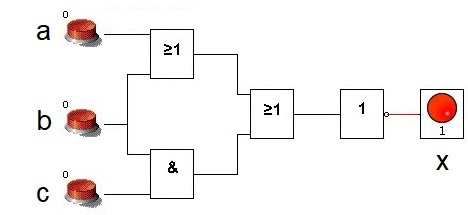
\includegraphics[width=\textwidth,align=t]{../99_Bilder/190308_SA.jpg}
			\end{minipage}
			\hfill
			\begin{minipage}{0.3\textwidth}
				Nach verschiedenen Tests wurden folgende Ergebnisse erreicht:\\
				\par\noindent
				\renewcommand{\arraystretch}{1.5}
				\begin{tabular}{|c|c|c|c|c|}
					\hline
					\rowcolor{codegray!15} \textbf{Test-Nr.} & \textbf{a} & \textbf{b} & \textbf{c} & \textbf{x}\\
					\hline
					\hline
					\fbox{1} & 0 & 0 & 0 & 1\\
					\hline
					\fbox{2} & 0 & 0 & 1 & 1\\
					\hline
					\fbox{3} & 0 & 1 & 0 & 0\\
					\hline
					\fbox{4} & 0 & 1 & 1 & 0\\
					\hline
					\fbox{5} & 1 & 0 & 0 & 0\\
					\hline
					\fbox{6} & 1 & 0 & 1 & 0\\
					\hline
					\fbox{7} & 1 & 1 & 0 & 1\\
					\hline
					\fbox{8} & 1 & 1 & 1 & 0\\
					\hline
				\end{tabular}\\
			\end{minipage}\\
			\par\noindent
			Welcher Test führt zu einem Ergebnis, das \textbf{nicht} der Logik der Schaltung entspricht?\\
			\par\noindent
			\rule{\textwidth}{0.1pt}\\
			
\includegraphics[width=0.5\textwidth]{../../empty.jpg}
		\end{framed}
		\begin{framed}
			\noindent
			Der Lagerplatz der \texttt{BIMS \& BUMS GmbH} wird mit einer speziellen Alarmanlage überwacht, die Umweltparameter für den Lagerraum sicherstellt. Um dies zu gewährleisten, messen die Sensoren Temperatur, Luftfeuchtigkeit und den Luftdruck. Alle drei Sensoren haben digitale Ausgänge, die beim Verletzen der vorgegebenen Grenzwerte von 0 auf 1 wechseln.\\
			\par\noindent
			Die digitale Schaltung erfüllt folgende Wahrheitstabelle:\\
			\par\noindent
			\begin{minipage}{0.25\textwidth}
				\renewcommand{\arraystretch}{1.5}
				\begin{tabular}{|c|c|c|c|}
					\hline
					\textbf{E1} & \textbf{E2} & \textbf{E3} & \textbf{A}\\
					\hline
					\hline
					0 & 0 & 0 & 0\\
					\hline
					0 & 0 & 1 & 0\\
					\hline
					0 & 1 & 0 & 0\\
					\hline
					0 & 1 & 1 & 1\\
					\hline
					1 & 0 & 0 & 1\\
					\hline
					1 & 0 & 1 & 1\\
					\hline
					1 & 1 & 0 & 1\\
					\hline
					1 & 1 & 1 & 1\\
					\hline
				\end{tabular}
				\begin{itemize}
					\item[E1] Temperatursensor
					\item[E2] Feuchtigkeitssensor
					\item[E3] Luftdrucksensor
				\end{itemize}
			\end{minipage}
			\hfill
			\begin{minipage}{0.7\textwidth}
				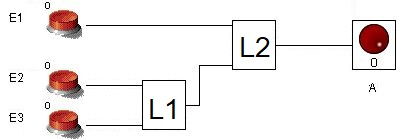
\includegraphics[width=\textwidth]{../99_Bilder/190308_SA_1.jpg}
			\end{minipage}\\
			\par\noindent
			Welche zwei logischen Schaltglieder sind an den Positionen \textbf{L1} und \textbf{L2} einzusetzen.\\
			\par\noindent
			\rule{\textwidth}{0.1pt}\\
			
\includegraphics[width=0.31\textwidth]{../../empty.jpg}
		\end{framed}
	\end{worksheet}
\end{document}